\chapter{Introduction}

Typical programming languages consist of plaintext tokens. These tokens
are used in grammar rules to specify which orderings of tokens are valid programs and
which are not.
\begin{figure}[!hbt]
	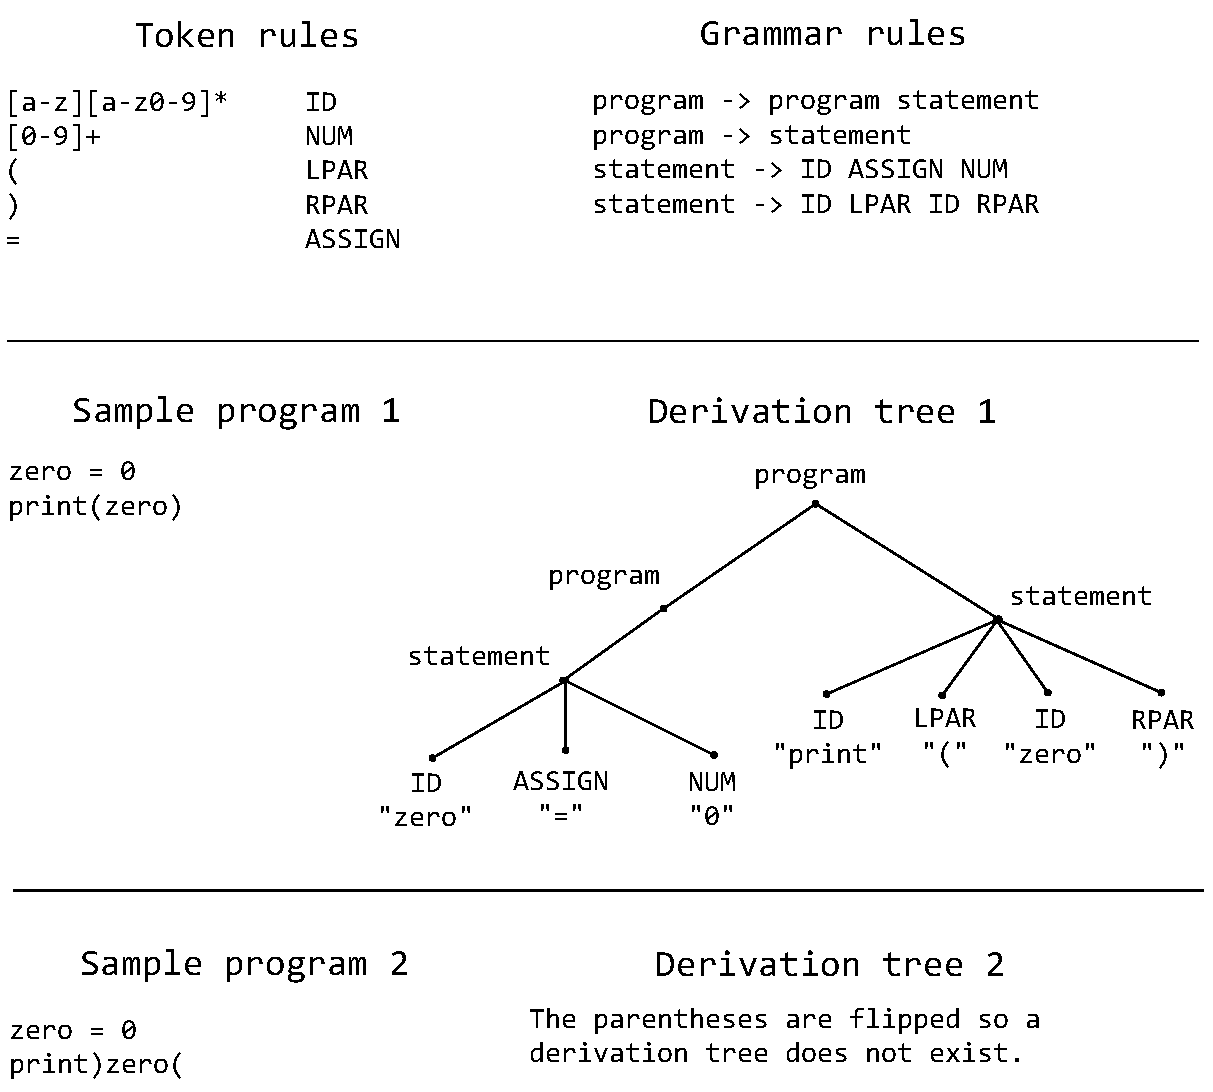
\includegraphics[width=\textwidth]{../img/tokens_and_grammar}
	\caption{Sample language definition with examples.}
	\label{fig:chap1:tokens_and_grammar}
\end{figure}

Figure \ref{fig:chap1:tokens_and_grammar} contains a set of token rules and grammar rules that define a~simple
language. \texttt{Sample program $1$} shows a valid program in this language with its respective derivation tree, while
\texttt{Sample program $2$} does not adhere to the grammar rules.
Even tough this example is trivial, it shows how the vast majority of programming languages are processed:
\begin{itemize}
\item \emph{Lexical analysis} splits the source code into tokens.
\item \emph{Syntax analysis} builds a tree based on the grammar rules. This tree is typically called an AST\footnote{Abstract Syntax Tree}
and it is similar to a derivation tree (Fig. \ref{fig:chap1:tokens_and_grammar} middle).
\item The AST is used to compile, interpret or transpile the source code.
\end{itemize}

Tokens do not have to consist of plaintext necessarily. Plaintext characters can be substituted with
images, videos, sounds, etc. In this thesis we construct a programming language with characters and some
of the keywords substituted with images and short looping videos (e.g., GIFs\footnote{Graphics Interchange Format is an image format that supports animations.}).
Figure \ref{fig:chap1:giflang_code} below shows the \texttt{Sample program 1} from Figure \ref{fig:chap1:tokens_and_grammar} written in
Giflang\footnote{We named the programming language developed in this thesis Giflang}.
\begin{figure}[!hbt]
	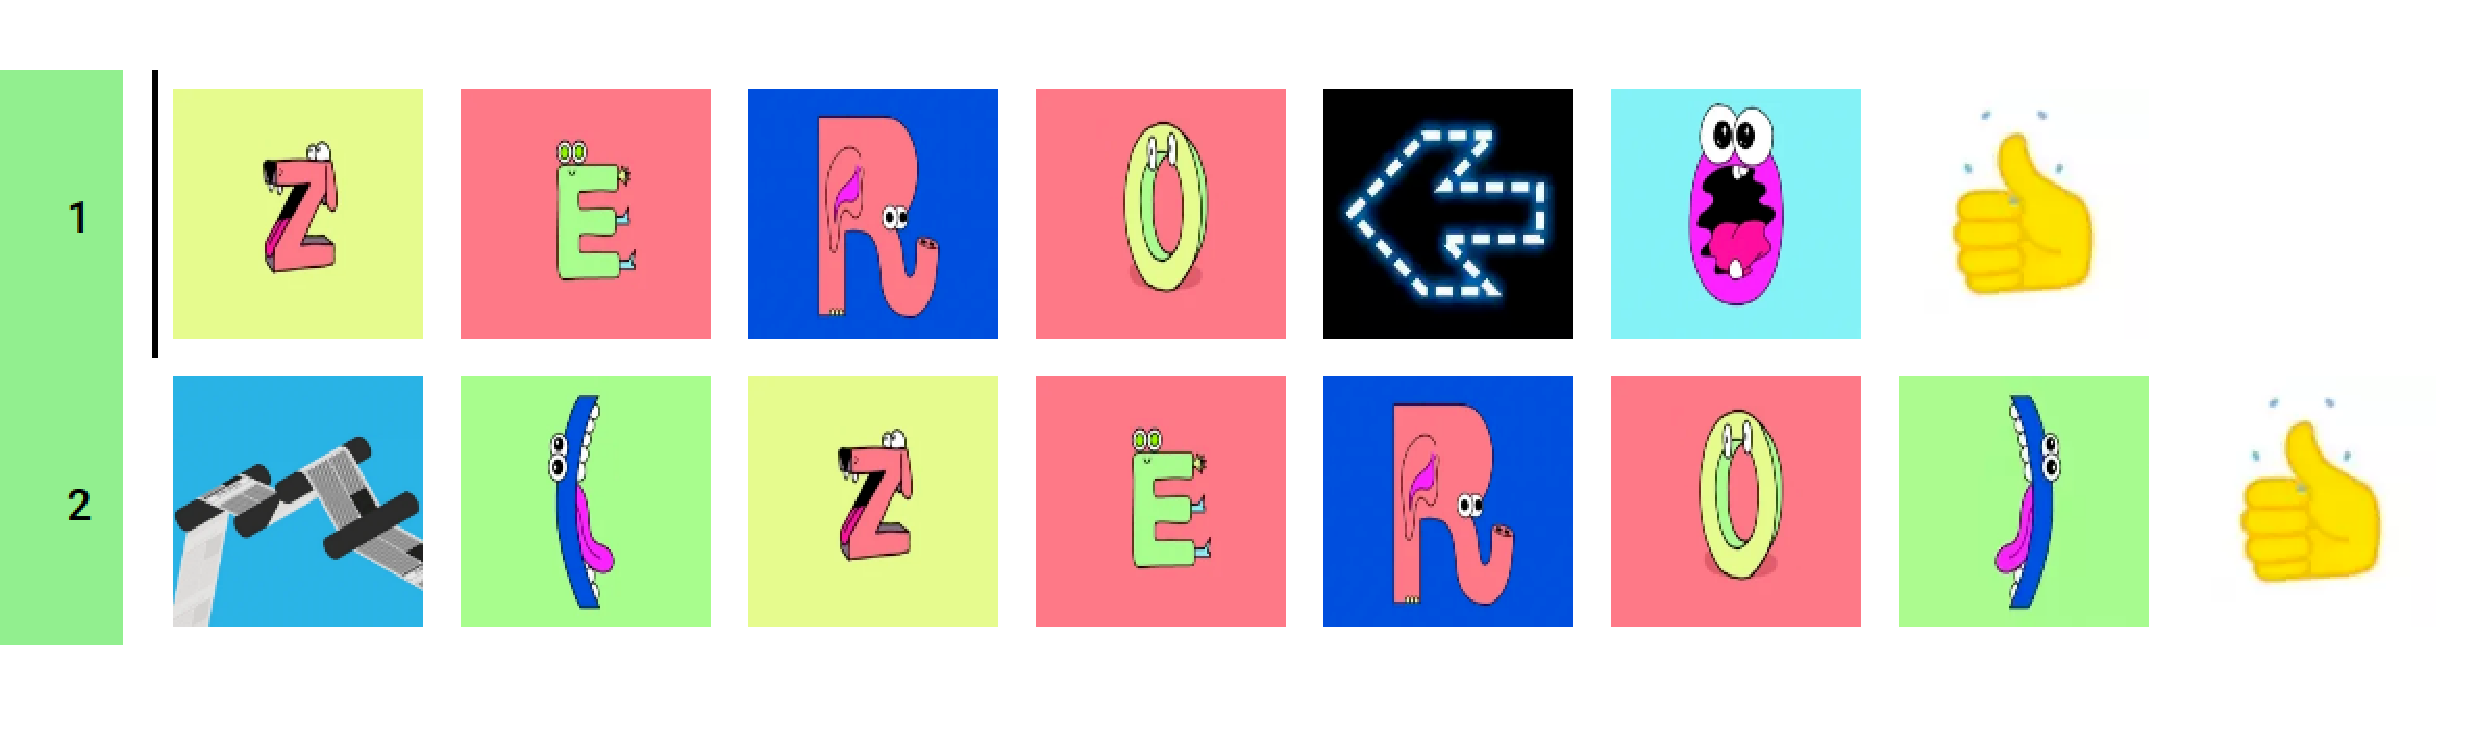
\includegraphics[width=\textwidth]{../img/giflang_code}
	\caption{Sample Giflang program}
	\label{fig:chap1:giflang_code}
\end{figure}

Characters and digits have their counterparts in Giflang. The assignment is represented with an arrow,
thumbs up is a semicolon and the \texttt{print} function is a single image containing paper. The exact choice of images used here is of course
irrelevant.

To store and parse programs like that, we need to define an intermediate format. The format can be for example
textual and the sample program from Figure \ref{fig:chap1:giflang_code} can be written as:
\begin{code}
Z;E;R;O; ASSIGN; 0; SEMICOLON;
PRINT; LPAR; Z;E;R;O; RPAR; SEMICOLON;
\end{code}

We discuss the intermediate format and the language design in Chapter \ref{chap3:language_design}. A language like this one is of
course impractical and hard to follow. We do not intent to create a language for practical use. Our $3$ main motivations for
creating Giflang are:
\begin{enumerate}
\item An image-based programming language like this does not exist yet. We show similar existing projects in Section \ref{chap1:related_work}. 
\item The author of this thesis co-organizes a Computer Science competition named Prask \cite{Prask}. After each semester we invite the best
contestants to a week-long programming camp filled with creative games, mostly related to Computer Science. We plan to incorporate Giflang into the games.
\item Allowing users to substitute images for their own can give younger users a feeling of creating ''their own language''.
\end{enumerate}

Since we use images instead of characters we need to implement our own IDE\footnote{Integrated Development Environment} to be able to
create and run Giflang programs.

To put it concisely, in this thesis we design a programming language with characters and some of the keywords substituted with images.
Additionally, we build an interpreter and an IDE for this language that both run in the browser. Goals mentioned here are described
more precisely in Section \ref{chap1:thesis_goals}. 

\section{Related work}
\label{chap1:related_work}
Visual programming languages are commonly used to introduce young audience to programming and this thesis was undeniably inspired by them.
A \emph{visual programming language} lets users create programs by manipulating program elements graphically rather than by specifying them
textually\footnote{Wikipedia}. Giflang is not a visual programming language as users can not manipulate graphical objects in its IDE, e.g.,
move them or connect them to other objects. It is also not a textual language per se as text is replaced by images. However, it is definitely closer
to a textual than a visual programming language.

\subsection{Emojicode}
An excerpt from the official documentation says that Emojicode \cite{Emojicode} is an open source, high-level, multi-paradigm programming language consisting of emojis.
It features Object-Orientation, Optionals, Generics and Closures.

Below is a `Hello World' program written in Emojicode:
\begin{figure}[!hbt]
	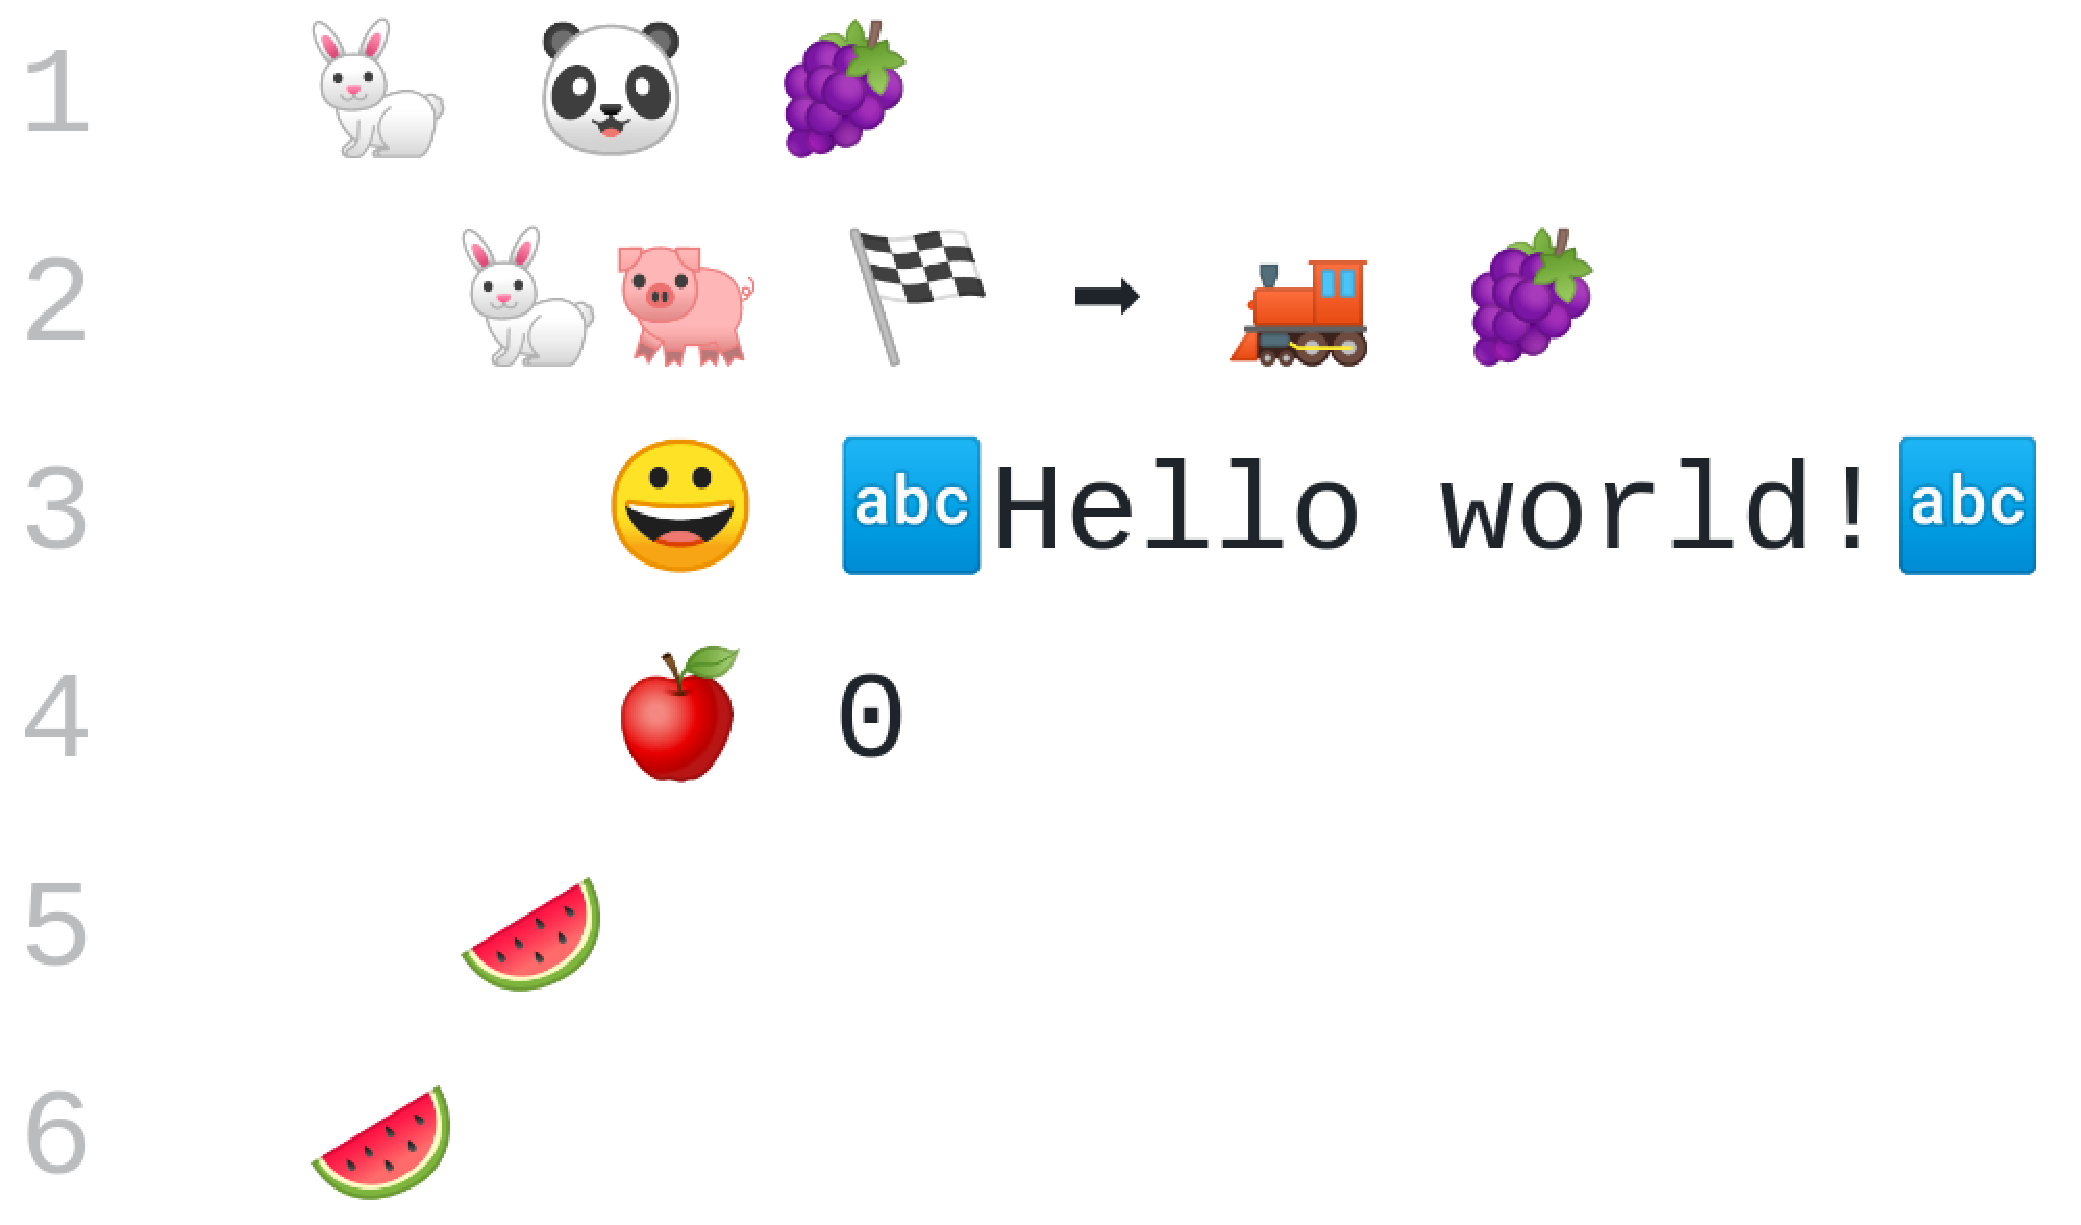
\includegraphics[width=0.5\textwidth]{../img/emojicode_helloworld}
	\label{fig:chap1:emojicode_helloworld}
\end{figure}

All built-in keywords and most of the special characters are replaced by emojis; for example, a raspberry is an opening curly brace \texttt{\{} in Emojicode.
However, as we can see in the `Hello World' program, not every character is replaced by an emoji. Additionally, users can not create their own emoji
mappings to keywords or characters. Creating Emojicode sources is simple as emojis are just Unicode characters and most of the modern text editors
have a good support for them.

Source code is compiled first to the LLVM IR\footnote{IR or Intermediate Language is a low-level programming language similar to assembly.} and then to
the machine code. With features such as compilation to an intermediate language, object-orientation, static typing and garbage collection, we can
say that Emojicode is similar to languages like C\# or Java.

The idea of Emojicode is similar to Giflang. However, since we are replacing characters and keywords with arbitrary images as
opposed to emojis, we have to use an intermediate textual format that maps to the images. Emojicode does not have this problem because emojis are
Unicode characters that can be represented in plaintext and parsed.

\subsection{JSFiddle}
JSFiddle \cite{JSFiddle} is a web IDE for testing and showcasing user-created and collaborational HTML, CSS and JavaScript code snippets, known as
'fiddles'\footnote{wikipedia copypaste}.

\begin{figure}[!hbt]
    \centering
	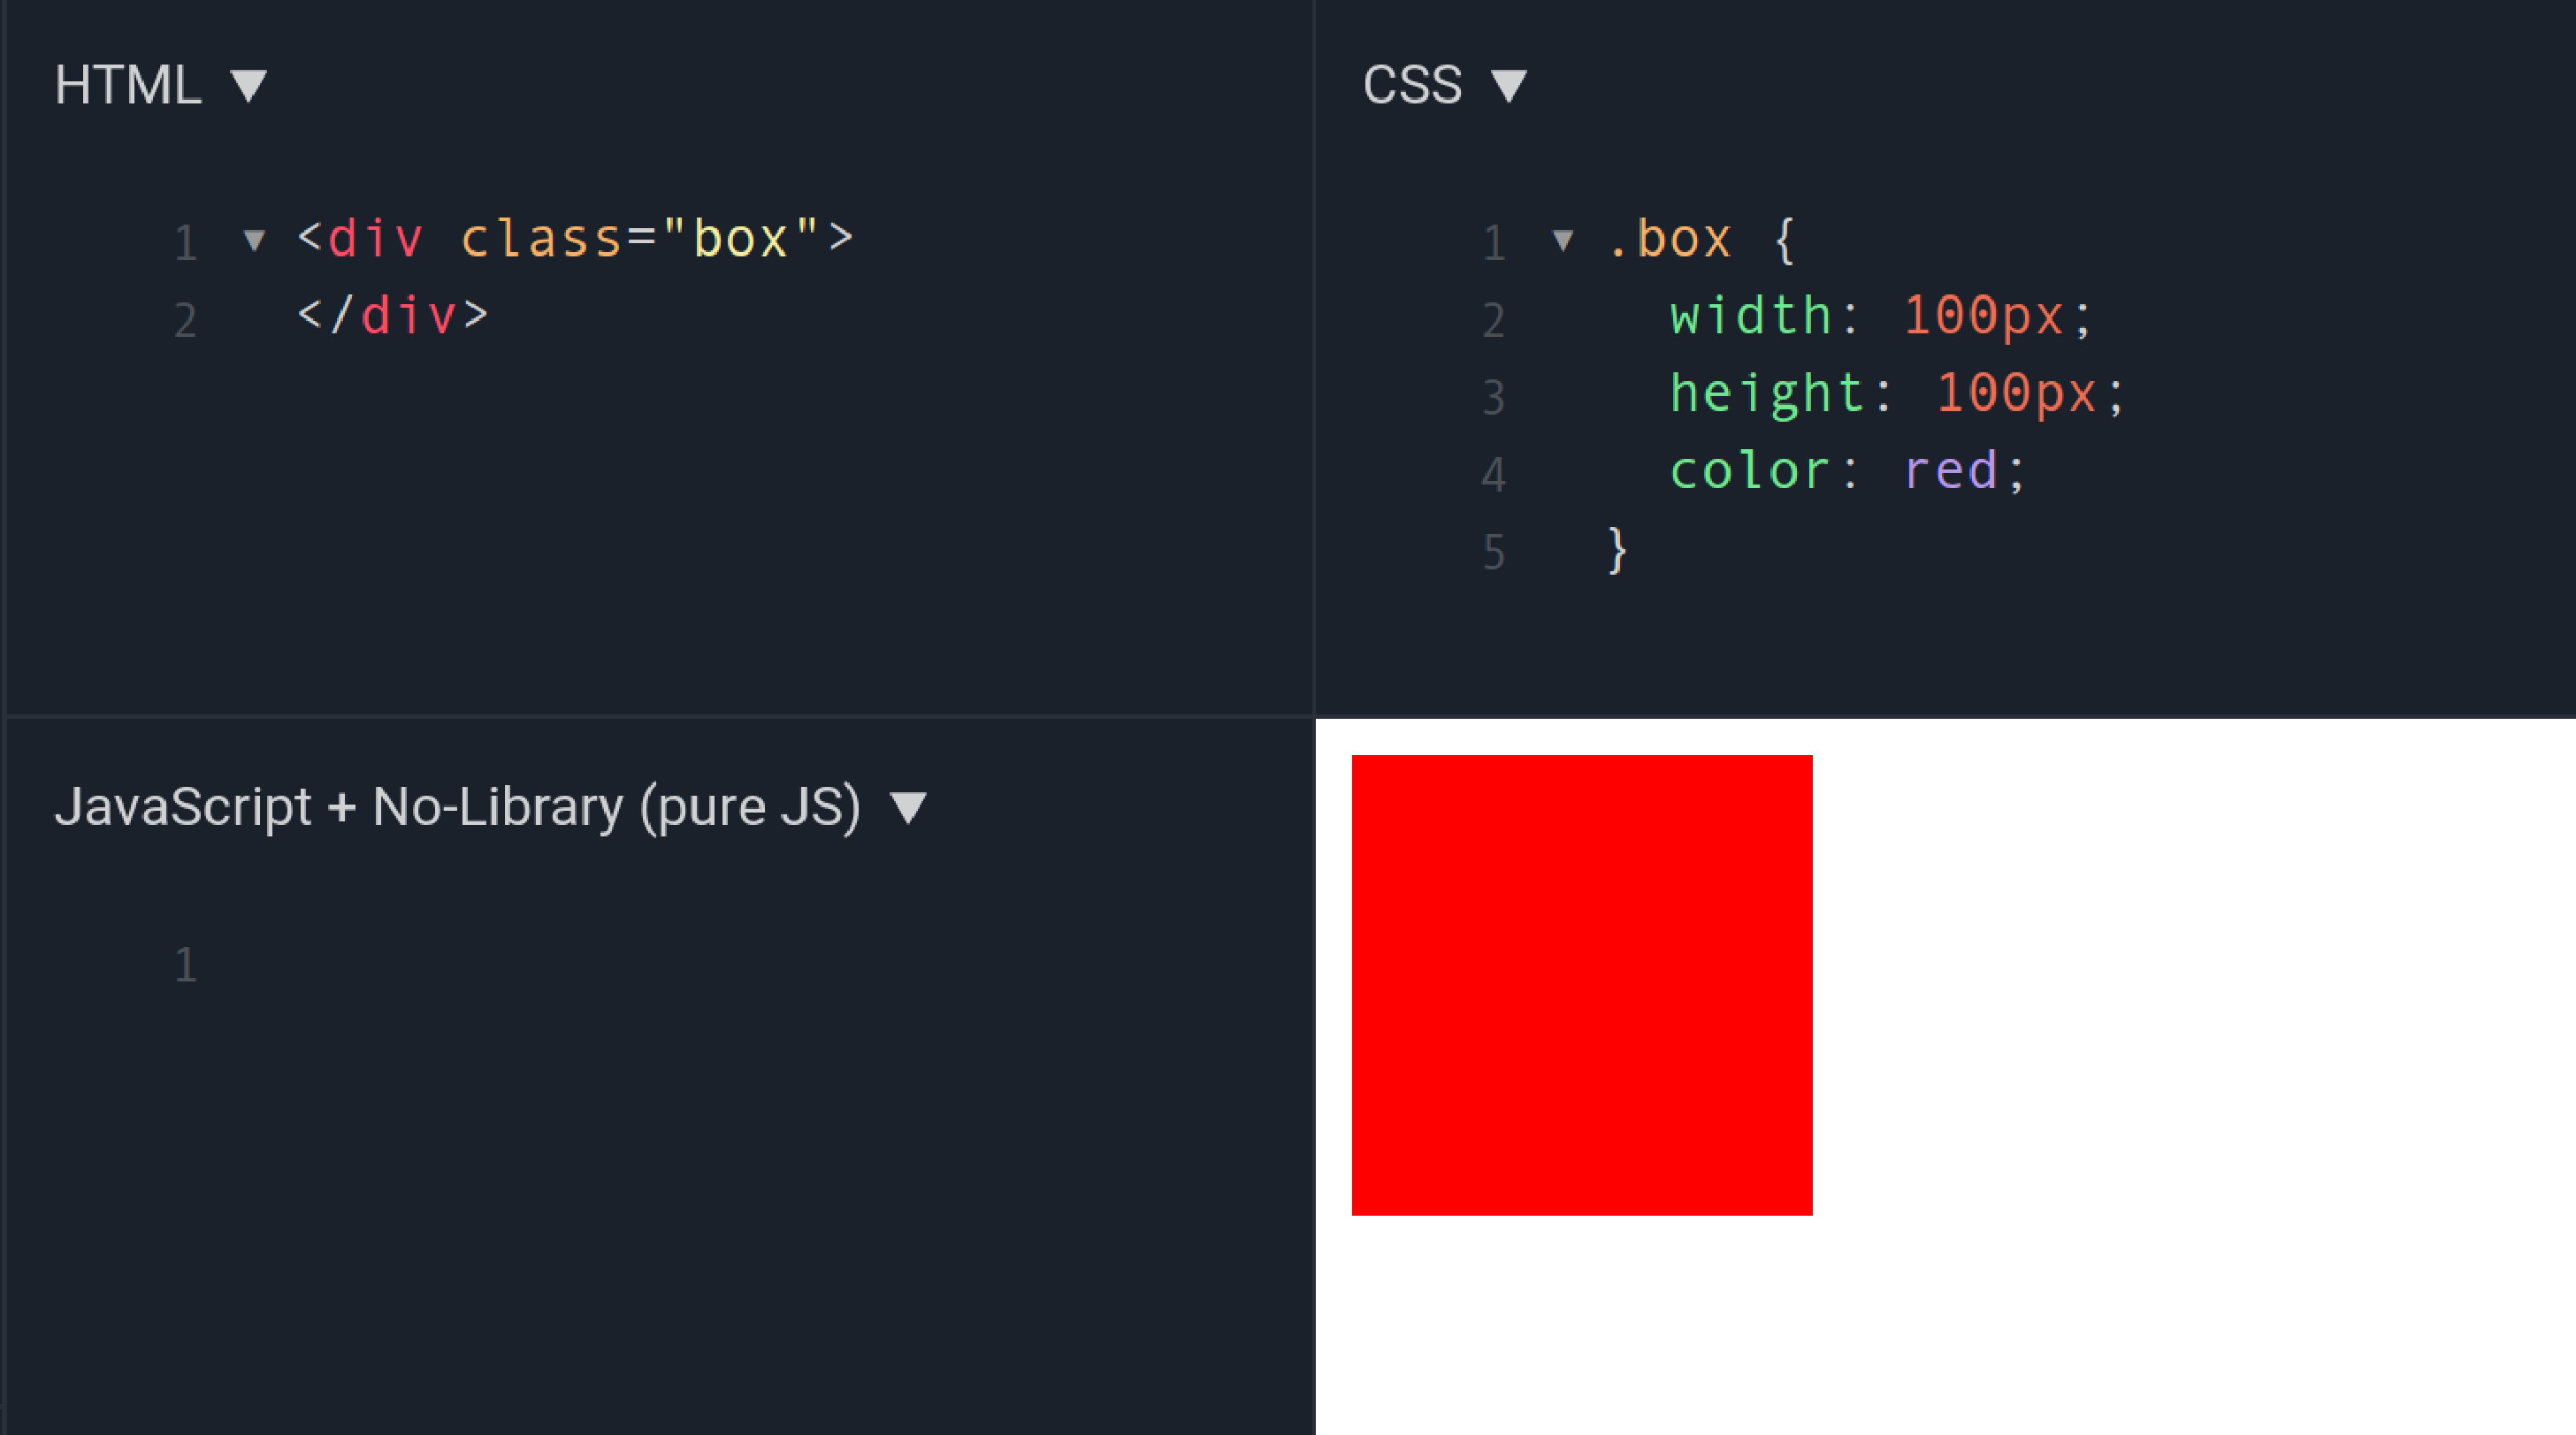
\includegraphics[width=\textwidth]{../img/jsfiddle}
	\caption{Sample fiddle}
	\label{fig:chap1:jsfiddle}
\end{figure}

Figure \ref{fig:chap1:jsfiddle} shows the core part of the JSFiddle UI. Users can input HTML, CSS and JavaScript, and the output is displayed in the
bottom right quadrant.

JSFiddle offers an interesting way of storing and forking\footnote{Forking an existing project means creating a new project based on the existing one.}
fiddles. First, users open a URL that contains an ID of a fiddle that should be loaded. Afterwards, users can edit the sources and run the fiddle.
At this point, the edited fiddle is not stored on the server. It is only stored after explicitly saved by the user. The save action gives the current
fiddle a new ID. This is how an existing fiddle can be forked. Any subsequent saves to the fork result in a new \emph{revision number} that is also
appended to the URL.

Revisions are numbered with natural numbers starting at 1. Each fiddle can be viewed at any of its revision numbers. Figure \ref{fig:chap1:jsfiddle_url}
below shows a URL with both an ID and a revision number.
\begin{figure}[!hbt]
    \centering
	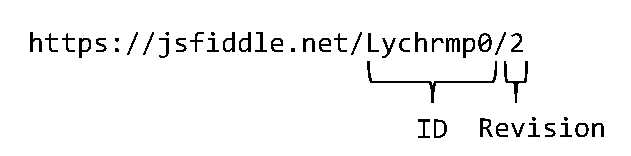
\includegraphics[width=0.5\textwidth]{../img/jsfiddle_url}
	\caption{A sample JSFiddle URL}
	\label{fig:chap1:jsfiddle_url}
\end{figure}

We got inspired by this simple storing and forking design and as mentioned in Section \ref{chap2:program_id} we use a similar approach in the Giflang IDE.

JSFiddle executes the code on the client side since all of the input languages, i.e., HTML, CSS and JavaScript, are natively supported in browsers.

\section{Thesis goals}
\label{chap1:thesis_goals}
In this section we define the scope of the thesis and formulate its precise goals. Primarily, we want to build an image-based programming language
with characters and keywords substituted with images. Since we want to make it easily accessible to users we want to implement its
IDE as a web application.

We split the goals into three major parts:
\begin{enumerate}
\item Giflang language design
   \begin{enumerate}[label=(\alph*)]
     \item Choose a suitable language type (object-oriented, functional, \ldots)
	 \item Define the syntax, semantics and a basic standard library
   \end{enumerate}
\item Client-side interpreter
   \begin{enumerate}[label=(\alph*)]
	 \item Design and implement an interpreter for Giflang
	 \item Support code-stepping with information about the current position in the source code, the call stack and the environment
	 \item Implement an API for a standard I/O
   \end{enumerate}
\item Web IDE
   \begin{enumerate}[label=(\alph*)]
     \item Design and implement an editor with characters replaced by images and support basic editing operations such as Delete,
     Backspace and cursor movement using the arrow keys
	 \item Allow specifying input to a running program and show its output using images
	 \item Support code-stepping with a visualization of the currently executed position in the source code
	 \item Allow storing programs on the server and loading the existing ones
	 \item Allow changing images in the mapping of images to characters and keywords
	\end{enumerate}
\end{enumerate}

Since the language is not meant for an actual application development we do not impose any performance goals on the interpreter; rather than that, we
focus on features like code-stepping with a highlighted source position.
